%!TEX root = main.tex

\chapter{Paradigma Bayesiano}

\begin{chapquote}{Dennis Lindley}
	``Dentro de cada no bayesiano, hay un bayesiano que lucha por salir.''
\end{chapquote}

\comment{extender un poco y suavizar más la entrada a temas duros, incluir un mini resumen del capitulo}
Lo que inicialmente nos motivó a estudiar el enfoque bayesiano son los llamados modelos no paramétricos: aquellos modelos que, a pesar de su nombre, tienen infinitos (o un número ilimitado de) parámetros que aumenta a medida de que observamos más datos. Algunos ejemplos comunes de modelos no paramétricos son los histogramas y las funciones de \emph{spline}, pero los basados en estadísticas bayesianas tienen una matemática más elegante y formal, coincidiendo en muchos aspectos con los procesos estocásticos. Un ejemplo de esto es el llamado proceso de Dirichlet, una distribución sobre distribuciones discretas, por lo que es muy útil en problemas de agrupamiento. Otro ejemplo distinguido con los procesos gaussianos, ya que se interpretan como distribuciones sobre espacios de funciones, muy útil en problemas de regresión. Este será el modelo de estudio en gran parte del libro.

\section{Modelos Bayesianos}

Consideremos las observaciones \(\calD = \{x_1, \dotsc, x_n\}\) de un espacio de datos \( \calX\) (por ejemplo \(\calX \subset \reals^q\)) y un conjunto de posibles modelos o medidas de probabilidades \(\calM \subseteq \calP(\calX)\), donde \(\calP(\calX)\) es el conjunto de medidas de probabilidad en \(\calX\). Por ejemplo, sea \(\calX=\{0,1\}\) tal que \[\calM = \{m_{\alpha} \in \calP(\calX) \mid m_\alpha(\{0\})=\alpha, m_\alpha(\{1\})=1-\alpha\text{, para } \alpha \in [0,1] \}\] es el espacio de distribuciones Bernoulli.


Entrenar un modelo, también conocido como selección de modelos, consiste en escoger un modelo \(m \in \calM\) que \emph{mejor} explique los datos \(\calD\) generados por \(m\), bajo algún criterio \cite{chipman2001practical}. Nosotros adoptamos el paradigma bayesiano, el cual provee de un marco probabilista para lidiar con la incertidumbre del modelo, en términos de una \emph{distribución a priori} \(\Pi\) sobre el espacio de modelos \(\calM\); referimos al lector a \cite{ghosal2017fundamentals, murphybook2012} y sus referencias para un trasfondo matemático de estadística bayesiana y métodos. Un desafío crítico en la perspectiva bayesiana es calcular la ley predictiva en \(\calX\), usualmente llamada la \emph{posterior predictiva} \cite{gelman2013bayesian}, desde la distribución posterior en \(\calM\).

Consideremos una medida de probabilidad \emph{a priori} \(\Pi\) sobre el espacio de modelos \(\calM\), es decir \(\Pi \in \calP(\calM)\). Siguiendo nuestro ejemplo consideremos \(\Pi\) sobre \(\calM\) de modo que \(\Pi(\{m_\alpha \mid \alpha \in A\}) = \lambda(A)\) para \(A \subseteq [0,1]\), donde \(\lambda\) denota la medida de Lebesgue. 


En virtud del Teorema de Bayes, la medida \emph{posterior} \(\Pi(\dd{m} \mid x_1, \dotsc, x_n)\) de modelos dados los datos \(\calD\), la cual se denota por simplicidad \(\Pi_n(\dd{m})\), está dada por
\begin{equation}\label{eq def Pi n}
	\Pi_n(\dd{m}) \coloneqq \frac{\Pi \left(x_1, \dotsc, x_n \mid m\right) \Pi \left(\dd{m}\right)}{\Pi \left(x_1, \dotsc, x_n\right)},
\end{equation}
donde \(\Pi(x_1, \dotsc, x_n) = \int_{\calM} \Pi(x_1, \dotsc, x_n \mid m) \Pi(\dd{m})\) es la verosimilitud marginal o \emph{evidencia} (constante con respecto a \(m\)), mientras que \(\calL_n(m) = \Pi  \left(x_1, \dotsc, x_n \mid m\right)\) es la función de \emph{verosimilitud}. Para nuestro ejemplo, denotando \(\bar{x} = \frac{1}{n}\sum_{i=1}^n x_i\), la función de \emph{verosimilitud} está dada por \(\calL_n(m_\alpha) = \alpha^{n \bar{x}} (1-\alpha)^{n (1-\bar{x})}.\)

\comment{parrafo: explicar intuición de lo recien explicado, puede ir antes o despues de la matematica dura}



\section{Enfoque Paramétrico}

En general supondremos que \(\calM \subseteq \calP_{\mathrm{ac}}(\calX)\), donde \(\calP_{\mathrm{ac}}(\calX)\) es el subconjunto de medidas absolutamente continuas con respecto a una misma medida \(\sigma\)-finita \(\lambda\) en \(\calX\) (por ejemplo la medida de Lebesgue). Como convención, usaremos la misma notación para un elemento \(m(\dd{x}) \in \calM\) y su densidad \(m(x)\) con respecto a \(\lambda\). \comment{luego de la explicación dura, explicarlo en palabras}

Se dice que \(\calM\) está finitamente parametrizado si hay un número \(k \in \naturals\), un conjunto \(\Theta \subseteq \reals^k\) llamado el espacio de parámetros, y una función (medible) \(\calI : \Theta \to \calP_{\mathrm{ac}}(\calX)\), llamado el mapeo de parametrización, tales que \(\calM = \calI(\Theta)\). En dicho caso denotamos \(m_\theta \coloneqq \calI(\theta)\). Siguiendo nuestro ejemplo, donde \(m_\alpha({0}) = \alpha\) y \(m_\alpha({1}) = 1-\alpha\), consideremos el espacio de parámetros \(\Theta = [0,1]\) y definimos dos mapas de parametrización: \(\calI_0(\theta) = m_\theta\) y \(\calI_1(\theta) = m_{\theta^{1/2}}\).

Dado \(p \in \calP(\Theta)\) una distribución a priori sobre el espacio de parámetros \(\Theta\), la medida \emph{push-forward}\footnote{«Que empuja hacia adelante» en español pero usaremos el anglicismo por comodidad.} a través del mapa \(\calI\) es la medida de probabilidad \(\Pi=\calI(p)\) sobre el espacio de modelos parametrizados \(\calM = \calI(\Theta)\), dado por \(\Pi(A)= p(\calI^{-1}(A))\) para \(A \in \mathcal{B}(\calM)\). Análogamente, como definimos el prior \(\Pi(\{m_\alpha \mid \alpha \in A\}) = \lambda(A)\), el prior inducido sobre \(\Theta\) corresponde a \(p(A) = \Pi(\calI(A)) \) para \(A \in \mathcal{B}(\Theta)\). Bajo la parametrización natural \(\calI_0\), el prior sobre \(\Theta\) es \(p_0(\theta) = \mathbf{1}_{\{\theta \in [0,1]\}}(\theta)\) y bajo \(\calI_1\) el prior inducido es \(p_1(\theta) = \frac{1}{2\theta^{1/2}}\mathbf{1}_{\{\theta \in [0,1]\}}(\theta)\).

Expresando la función de verosimilitud \(\calL_n(m)\) en términos del parámetro \(\theta\) sujeto a \(\calI(\theta) = m_\theta\), obtenemos de la ecuación \eqref{eq def Pi n} la densidad posterior estándar sobre el espacio de parámetros,  
\begin{align*}
	p_n(\theta) := p(\theta| x_1,\dots, x_n) = \frac{p(x_1,\dots, x_n \mid \theta) p(\theta)}{p(x_1, \dots, x_n)}.
\end{align*}

Si el espacio de modelos \(\calM\) es finitamente parametrizable, entrenar un modelo significa en encontrar los \emph{mejores} parámetros \(\theta \in \Theta\). El enfoque frecuentista es indiferente al prior sobre los modelos, ya que para encontrar los \emph{mejores} parámetros \(\theta \in \Theta\) se resuelve a través del estimador de máxima verosimilitud (MLE por sus siglas en inglés), dado por
\[\hat\theta_{\mathrm{MLE}} \in \argmax_{\theta \in \Theta} \calL_n(\theta),\]
donde \(\calL_n(\theta) = p(x_1, \dotsc, x_n \mid \theta)\) es la función de verosimilitud. En algunos casos particulares el valor extremo es único, pero en general hay muchos óptimos locales y globales. Un truco numérico se basa en considerar maximizar el logaritmo de la función de verosimilitud, usualmente denotada como \(\ell_n(\theta) = \log \calL_n(\theta)\), y como el logaritmo es una función estrictamente creciente, maximizar la función de verosimilitud es equivalente a maximizar la función de log-verosimilitud, o equivalentemente minimizar la función de log-verosimilitud negativa.

Considerando el prior, análogamente al MLE el estimador de \emph{máximo a posteriori} (MAP por sus siglas en inglés) es definido como
\begin{align*}
	\hat\theta_{MAP} \in \argmax_{\theta \in \Theta} p_n(\theta).
\end{align*}

Dado que la verosimilitud marginal \(p(x_1,...,x_n)\) es constante para \(\theta\), el estimador MAP puede ser calculado por el funcional equivalente
\begin{align*}
	\hat\theta_{MAP} \in \argmax_{\theta \in \Theta} \ell_n(\theta) + \log p(\theta).
\end{align*}
Bajo el punto de vista frecuentista, el término \emph{log prior} \(\log p(\theta)\) puede ser interpretado como un término de regularización, por lo que MAP es un estimador regularizado de MLE. En el caso que \(p(\theta)\) es \emph{no informativo}, es decir \(p(\theta) \propto 1\), el estimador MAP coincide con el MLE.

El enfoque de MAP es computacionalmente atractivo ya que reduce el problema de estimación a un problema de optimización en un espacio finito dimensional. Sin embargo, el rendimiento de este método podría ser muy sensible a la elección de la condición inicial utilizada en el algoritmo de optimización \cite{wright1999numerical}. Este problema es un inconveniente crítico, ya que las funciones de verosimilitud sobre los parámetros pueden poblarse con numerosos óptimos locales. 

El segundo inconveniente de este método es que no captura la información global del espacio modelo, lo que podría resultar en un sobreajuste de la distribución predictiva. De hecho, la moda a menudo puede ser un resumen muy pobre o una elección atípica de la distribución posterior (por ejemplo, la moda de una densidad exponencial \(Exp(\lambda)\) es \(0\), independiente de su parámetro de tasa \(\lambda\)). 

Otro fallo grave de la estimación MAP es su dependencia de la parametrización, es decir el modelo estimado que obtenemos depende de la elección del mapeo \(\calI:\Theta \to \calM\) \cite{murphybook2012}\footnote{El estimador MLE no sufre de este problema ya que la verosimilitud es una función, no una densidad de probabilidad y satisface la propiedad de invarianza \cite[Theorem 7.2.1]{mukhopadhyay2000probability}. }. Para nuestro ejemplo denotando \(\alpha = \theta\), bajo la parametrización natural \(\calI_0\) tenemos que el funcional, su derivada y el modelo óptimo corresponden a:
\begin{align*}
	J_0(\alpha) &= n\bar{x}\log \alpha + n(1-\bar{x})\log(1-\alpha), \\
	\partial_\alpha J_0(\alpha) &= \frac{n\bar{x}}{\alpha} - \frac{n(1-\bar{x})}{1-\alpha}, \\
	\hat{m}_0 &= m_{\bar{x}}.
\end{align*}
Análogamente, bajo la parametrización \(\calI_1\) y denotando \(\alpha = \theta^{1/2}\) tenemos que.
\begin{align*}
	J_1(\alpha) &= c + (n\bar{x} -1)\log \alpha + n(1-\bar{x})\log(1-\alpha),\\
	\partial_\alpha J_1(\alpha) &= \frac{n\bar{x}-1}{\alpha} - \frac{n(1-\bar{x})}{1-\alpha},\\
	\hat m_1 &= m_{\left(\frac{n\bar{x}-1}{n-1}\right)}.
\end{align*}

El enfoque bayesiano permite obtener estimadores que no sufren de los problemas recién descritos, y es a través de integrar sobre todo el espacio de modelos/parámetros.

\section{Estimadores de Bayes}
\label{sec bayes estimators}

Volviendo al caso general, una función de pérdida \(L:\calM \times \calM \to \mathbb{R}\) es un funcional no negativo. Interpretamos \(L(m_\star, \bar{m})\) como el costo de seleccionar el modelo \(\bar{m} \in \calM\) cuando el verdadero modelo es \(m_\star \in \calM\). Con una función de pérdida y la distribución posterior sobre los modelos, definimos el riesgo de Bayes (o pérdida esperada\footnote{En la literatura, el riesgo de Bayes se refiere a la pérdida esperada con una medida fija, pero en nuestro contexto, está implícito que las expectativas y los estimadores son con respecto a la medida posterior \(\Pi_n\).}) \(R(\bar{m}|D)\) y el estimador de Bayes \(\hat{m}_L\) de la siguiente manera:
\begin{eqnarray}
	\label{eq hat m abstract}
	R_L(\bar{m}|D) &:=&  \int\limits_{\calM} L(m,\bar{m})\Pi_n(\dd m) \, ,\\
	\hat{m}_L &\in&\textstyle \argmin\limits_{\bar{m} \in \calM} R_L(\bar{m}|D). 
\end{eqnarray}

En el enfoque paramétrico, cualquier función de pérdida \(L\) induce un funcional \(l : \Theta \times \Theta \to \mathbb{R}\) (y viceversa) definido por
\(l(\theta_\star,\bar{\theta}) = L (m_{\theta_\star}, m_{\bar{\theta}})\), interpretado como el costo de elegir el parámetro \(\bar{\theta}\) cuando el parámetro verdadero es \(\theta_\star\). El riesgo de Bayes \cite{berger2013statistical} de \(\bar{\theta} \in \Theta\) y su estimador de Bayes \(\hat{\theta}_{l}\) están definidos por
\begin{eqnarray}
	\label{eq:param_bayes_risk}
	\textstyle R_{l} (\bar{\theta}|D) &:=& \int\limits_{\Theta} l (\theta ,\bar{\theta})p_n(\dd\theta)=  \int\limits_{\calM} L(m,\bar{m})\Pi_n(\dd m),\\
	\hat{\theta}_{l} &\in&\argmin_{\bar{\theta} \in \Theta }R_{l}(\bar{\theta}|D).
\end{eqnarray}

A modo de ilustración, considere la función de pérdida 0-1 definida como \(l_{0-1}(\theta ,\bar{\theta}) = 1-\delta_{\bar{\theta}}(\theta)\). Su riesgo de Bayes es \(R_{l_{0-1}}(\bar{\theta}|D) = 1-p_n(\bar{\theta})\), por lo que el estimador de Bayes correspondiente es la moda de \(p_n(\bar{\theta})\), es decir \(\hat{\theta}_{l_{0-1}} = \hat{\theta}_{MAP}\). Para cantidades de valor continuo, el uso de la función de pérdida cuadrática \(l_{2}( \theta ,\bar{\theta}) =\Vert \theta -\bar{\theta}\Vert_{2}^{2}\) es a menudo preferido, y su estimador de Bayes es la media posterior \(\hat{\theta}_{l_{2}}=\int_{\Theta }\theta p_n(\dd\theta)\). Usando la función de pérdida de valor absoluto \(l_{1}( \theta ,\bar{\theta}) =\Vert \theta -\bar{\theta}\Vert_{1}\), esta produce el estimador de la mediana posterior \cite{stroock2010probability} .

El uso de estimadores generales de Bayes en modelos parametrizados permite una elección más rica de criterios para la selección de modelos al integrar información global del espacio de parámetros al tiempo que proporciona una medida de incertidumbre a través del valor de riesgo de Bayes. 

Sin embargo, este enfoque también puede presentar los problemas relacionados con la parametrización, como la sobreparametrización del espacio modelo (decimos que \(\calI\) sobreparametriza \(\calM\) si \(\calI(\theta):\Theta \to \calM\) no es biyectiva). Esto último podría resultar en una distribución posterior multimodal sobre los parámetros. Por ejemplo, tome \(\mathcal{X}=\Theta = \mathbb{R}\), \(m_\star=\mathcal{N}(\mu,1)\) con \(\mu > 0 \) y \(\calI(\theta)=\mathcal{N}(|\theta|, 1)\). Si elegimos un prior simétrico, por ejemplo \(p(\theta)=\mathcal{N}(0,1)\), entonces con suficientes datos la distribución posterior es simétrica con modos cerca de \(\{\mu,-\mu\}¸\), por lo que ambos estimadores \(l_{1}\) y \(l_{2}\) están cerca de \(0\).

Para abordar los problemas anteriores, es mejor utilizar criterios de selección no paramétricas través de funciones de pérdida que comparan directamente las distribuciones en lugar de sus parámetros. Dado que tanto \(L\) como \(\Pi_n\) operan directamente en el espacio del modelo, el aprendizaje del modelo de acuerdo con las ecuaciones anteriores no depende de los aspectos geométricos de los espacios de parámetros. Además, este punto de vista nos permite definir funciones de pérdida en términos de varias métricas/divergencias directamente en el espacio \(\calP(\calX)\), y por lo tanto mejorar el marco de estimación bayesiano clásico. Encontrar los estimadores corresponden a encontrar la llamada media de Fréchet o baricentro \cite{panaretos2017frechet}.

Sea \(\calM = \calP_{ac}(\calX)\) y considere la función de pérdida \(L_{2}(m,\bar{m}) = \frac{1}{2}\int_{\calX}\left( m(x)-\bar{m}(x)\right) ^{2}\lambda (\dd x)\), entonces el estimador de Bayes correspondiente corresponde al \emph{modelo bayesiano promedio}:
\begin{align*}
	\label{eq:model_average}
	\bar{m}(x) := \mathbb{E}_{\Pi_n}[m] = \int_{\calM}m(x)\Pi_n(\dd m) = \int_{\Theta}m_\theta(x)p_n(\dd \theta) \approx \frac{1}{N}\sum_i^N m_{\theta_i}(x).
\end{align*}


\section{Modelos Bayesianos de Regresión}

En diversos campos, como las finanzas, la física y la ingeniería, podemos encontrar entornos donde las observaciones están indexadas por tiempo o espacio y transmiten alguna estructura de dependencia oculta que pretendemos descubrir. Esta configuración corresponde a un problema de regresión que se puede resumir de la siguiente manera.

Sean \(n \in \naturals\) observaciones de entrada y salida \((\bft, \bfx) = \{(t_i, x_i)\}_{i=1}^n\) donde \(t_i \in \calT \subseteq \reals^T\), \(T \in \naturals\) y \(x_i \in \calX \subseteq \reals^m\) para \(i = 1, \dotsc, n\) con \(m,T \in \naturals\), el problema de regresión tiene como objetivo estimar el \emph{mejor} predictor \(f : \calT \to \calX\), tal que los \(f(t_i)\) estén \emph{cerca} de los \(x_i\), donde los términos \emph{mejor} y \emph{cerca} están dados por el criterio de optimización escogido. 

Para resolver este problema de regresión, deseamos un modelo que pueda interpolar y extrapolar, calcular estimaciones puntuales, barras de error y generar funciones plausibles, como vemos en la Fig. \ref{fig:regression_problem}. Una solución ampliamente utilizada para este problema de regresión es el proceso gaussiano \cite{rasmussen06}, también conocido como \emph{kriging} \cite{stein2012interpolation,cressie1990origins}, el cual es un caso de modelo bayesiano no paramétrico.

\begin{figure}[!h]
	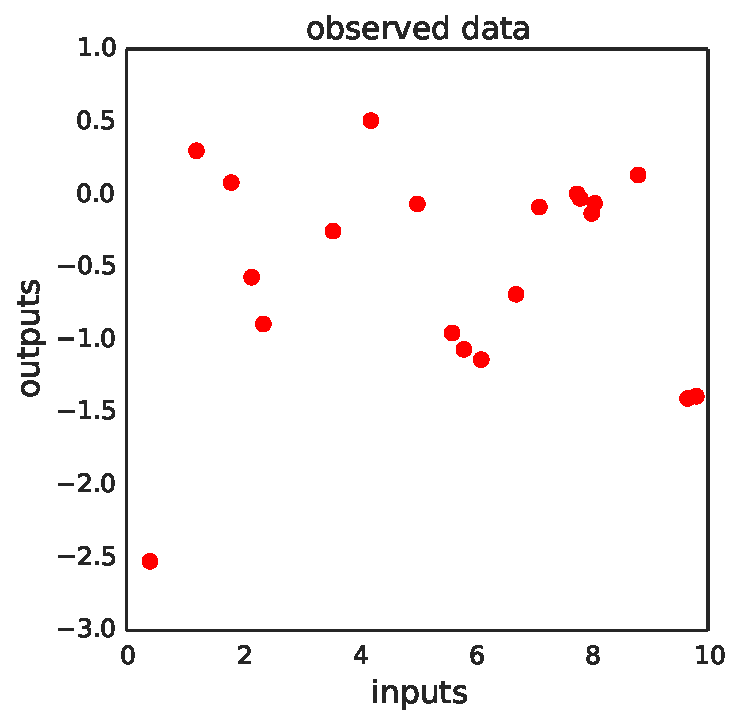
\includegraphics[width=0.24\textwidth]{reg_1}
	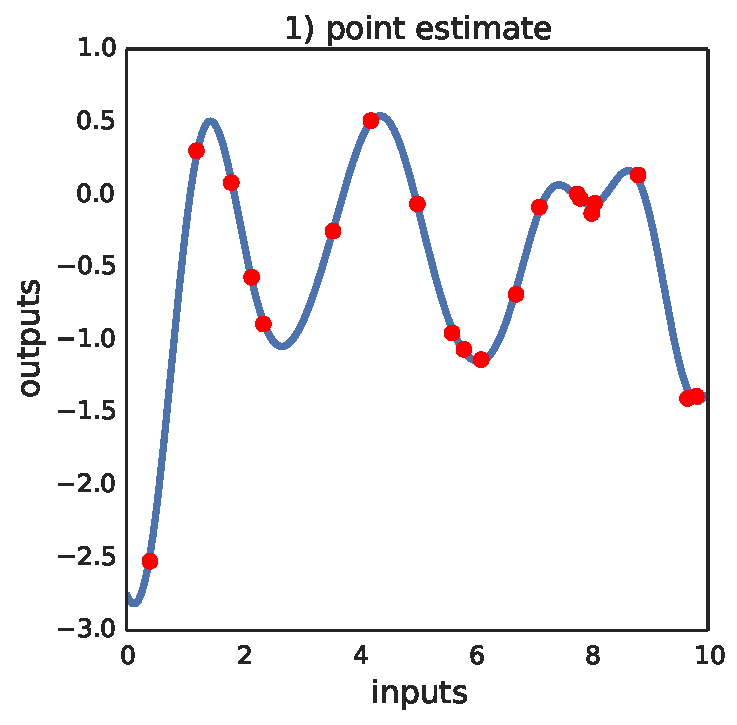
\includegraphics[width=0.24\textwidth]{reg_2}
	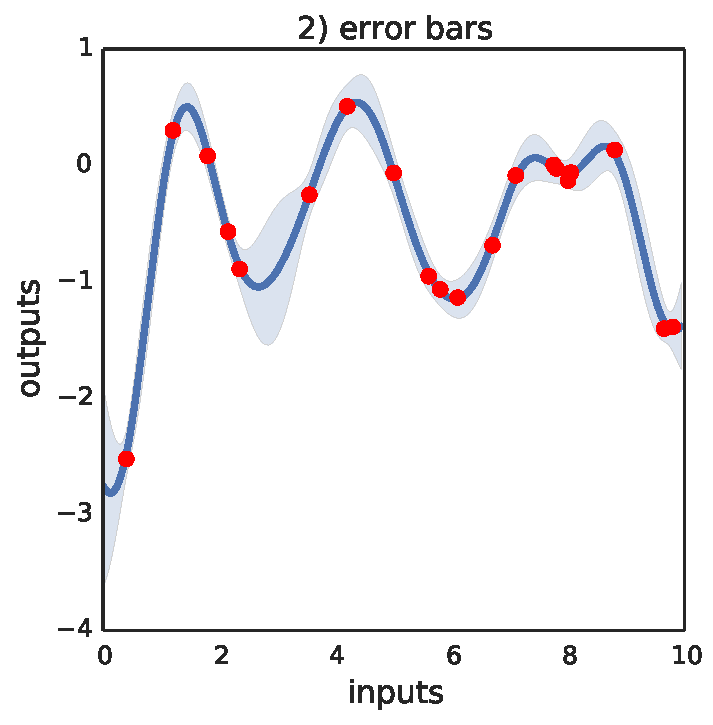
\includegraphics[width=0.24\textwidth]{reg_3}
	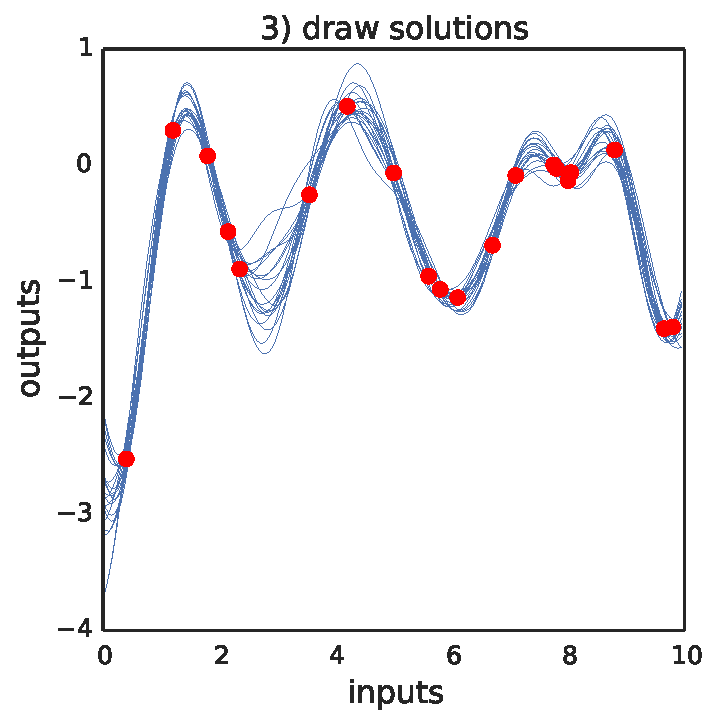
\includegraphics[width=0.24\textwidth]{reg_4}
	\caption{De izquierda a derecha, se muestran datos, estimaciones puntuales, barras de error, y funciones plausibles.}
	\label{fig:regression_problem}
\end{figure}

\section{Modelos Bayesianos Jerárquicos}
\label{sec:hierarchical}

\begin{figure}[h]
	\centering
	\tikz{ 
		\node[obs] (x) {\(\bfx\)};
		\node[obs, right=of x] (t) {\(\bft\)};
		\node[latent, above=of x, yshift=-0.3cm] (theta) {\(\theta\)};
		\node[latent, above=of theta, yshift=-0.3cm] (omega) {\(\omega\)};
		\edge {omega} {theta};
		\edge {theta, t} {x};
		% Plates
		\plate[inner sep=0.3cm, yshift=0.2cm]  {xt} {(t)(x)} {\(\calD\)};
	}
	\hspace{5em}
	\tikz{
		\node[obs] (x) {\(\bfx\)};
		\node[obs, right=of x] (t) {\(\bft\)};
		\node[det, above=of x, yshift=-0.3cm] (theta) {};
		\node[latent, above=of theta, yshift=-0.3cm] (omega) {\(\omega\)};
		\edge {omega} {theta};
		\edge {theta, t} {x};
		% Plates
		\plate[inner sep=0.3cm, yshift=0.2cm]  {xt} {(t)(x)} {\(\calD\)} ;
	}
	\caption{Izquierda: representación gráfica de un modelo bayesiano jerárquico para regresiones, con \emph{hiperparámetros} \(\omega\), \emph{parámetros} \(\theta\) y datos de entrada/salida \(\bft, \bfx\). Derecha: representación gráfica del mismo modelo bayesiano jerárquico, pero integrando los parámetros \(\theta\).}
	\label{fig:hierarchical_model}
\end{figure}

Un \emph{modelo bayesiano jerárquico} está escrito en múltiples etapas o niveles, donde toda la incertidumbre está modelada en términos probabilísticos y se permite utilizar el teorema de Bayes entre dichas etapas de diferente nivel de abstracción. 

Dado un espacio de modelos parametrizado \(\calM = \calI(\Theta)\), consideremos \(p(\theta) \in \calP(\Theta)\) una distribución a priori sobre los parámetros. Si este prior está a la vez parametrizado por \(\omega \in \Omega\), llamados \emph{hiperparámetros}, entonces podemos fijar un \emph{hiperprior} \(p(\omega) \in \calP(\Omega)\) sobre ellos. 

En principio, se puede iterar el proceso: si el hiperprior a su vez tiene parámetros, a estos se les puede llamar hiper-hiperparámetros, y así. Sin embargo, en algún punto debemos parar. 

En la Fig. \ref{fig:hierarchical_model} (izquierda), se presenta un esquema de regresión de dos etapas, donde \(\calD = (\bft, \bfx)\) son datos de entrada/salida y la distribución conjunta es \[p(\bfx, \bft, \theta, \omega) = p(\bfx, \bft \mid \theta, \omega) p(\theta \mid \omega) p(\omega).\]

Fijando un prior \emph{no informativo} sobre \(\bft\), es decir, \(p(\bft \mid \theta, \omega) \propto 1\), con esto la distribución posterior de los parámetros \(\theta\) dado \(\bft,\bfx,\omega\) está dada por
\begin{equation*}
	p(\theta \mid \bfx, \bft, \omega) = \frac{p(\bfx \mid \bft, \theta, \omega) p(\theta \mid \omega)}{p(\bfx \mid \bft, \omega)},
\end{equation*}
donde \(p(\bfx \mid \bft, \theta, \omega) \) es la verosimilitud de \(\theta\), \(p(\theta \mid \omega)\) es el prior de \(\theta\) y la verosimilitud marginal es
\begin{equation*}
	p(\bfx \mid \bft, \omega) = \int_{\Theta} p(\bfx \mid \bft, \theta, \omega) p(\dd{\theta \mid \omega}).
\end{equation*}

Para un hiperparámetro fijo \(\omega\), podemos entrenar el modelo parametrizado por \(\theta\) con cualquier estimador de Bayes, como el máximo a posteriori \(\hat{\theta}_{\mathrm{MAP}} \in \argmax_{\theta \in \Theta} p(\theta \mid \bfx, \bft, \omega)\) o la media posterior \(\hat{\theta}_{l_2} = \int_{\Theta} \theta p(\dd{\theta \mid \bfx, \bft, \omega})\). Adicionalmente, en el contexto de los modelos bayesianos jerárquicos, podemos calcular la \emph{distribución predictiva posterior} de \(\bfxo\) para nuevas entradas \(\bfto\), que está dada por
\begin{equation*}
	p(\bfxo \mid \bfto, \bfx, \bft, \omega) = \int_{\Theta} p(\bfxo \mid \bfto, \theta, \omega) p(\dd{\theta \mid \bfx, \bft, \omega}),
\end{equation*}
que coincide con el \emph{modelo bayesiano promedio} en \(\theta\), es decir
\begin{align}
	\bar m(\bfxo \mid \bfto, \omega)	&= \int_{\Theta} m_{\theta}(\bfxo \mid \bfto, \omega) p(\dd{\theta \mid \bfx, \bft, \omega}) \nonumber \\
										&= \int_{\Theta} p(\bfxo \mid \bfto, \theta, \omega) p(\dd{\theta \mid \bfx, \bft, \omega}) \nonumber\\
										&= p(\bfxo \mid \bfto, \bfx, \bft, \omega).
\end{align}

Notemos que el \emph{modelo bayesiano promedio} \(\bar{m}(\bfxo \mid \bfto, \omega)\) depende solo de \(\omega\), dado que \emph{desintegramos} el parámetro \(\theta\), por lo que debemos \emph{escoger} el hiperparámetro \(\omega\). Para esto, siguiendo el paradigma bayesiano ilustrado en la Figura \ref{fig:hierarchical_model} (derecha), calculamos la distribución posterior de \(\omega\) dado \(\bft, \bfx\) como sigue:
\begin{equation*}
	p(\omega \mid \bfx, \bft) = \frac{p(\bfx \mid \bft, \omega) p(\omega)}{p(\bfx \mid \bft)},
\end{equation*}
donde \(p(\bfx \mid \bft, \omega)\) es la \emph{verosimilitud} de \(\omega\) (a tono con la verosimilitud marginal relacionada a \(\theta\)), \(p(\omega)\) es el prior de \(\omega\) y \(p(\bfx \mid \bft)\) es la verosimilitud marginal relacionada a \(\omega\).

Dado \(p(\omega \mid \bfx, \bft)\), también podemos escoger el modelo (hiper-)parametrizado por \(\omega\) con cualquier estimador de Bayes. En la etapa de hiperparámetros, es normal usar el estimador máximo a posteriori \(\hat{\omega}_{\mathrm{MAP}}\), denotado MAP-II para diferenciarlo del estimador del parámetro MAP \(\hat{\theta}_{\mathrm{MAP}}\), el cual denotamos MAP-I. La razón de esto es que es más común tener posteriores de \(\omega\) más puntiagudas, es decir concentradas en torno a un punto, que usualmente coincide con el MAP-II.

El hecho de integrar los parámetros es lo que distingue el enfoque bayesiano de inferencia con respecto a los enfoques basados en optimización, ya que la verosimilitud marginal incorpora un equilibrio entre ajuste y complejidad.

Si queremos un estimador de Bayes diferente, como el \emph{modelo promedio de hiperparámetros}, nos enfrentamos a un posible problema: las integrales con respecto a \(p(\omega \mid \bfx, \bft)\) son intratables. Sin embargo, podemos aproximarlas por muestras de la distribución usando métodos bayesianos de muestreo, que veremos en la siguiente sección.

El marco teórico introducido se utiliza ampliamente para definir modelos \emph{no paramétricos}, es decir, modelos sin un número fijo de parámetros y que pueden crecer con los datos. Podemos distinguir un modelo no paramétrico que tiene muchas propiedades matemáticas que lo hacen versátil y flexible, especialmente para trabajos de regresión basadas en la distribución gaussiana.

\section{Inferencia Bayesiana}
\comment{explicar la intuición de por que queremos estimar esa integral}
Como vimos en las secciones anteriores, estamos interesados en calcular integrales con respecto a la distribución posterior de parámetros \(p_n(\theta) = \frac{p(x_1,\dots, x_n \mid \theta) p(\theta)}{p(x_1, \dots, x_n)}\), donde la constante de normalización o \emph{evidencia} \(p(x_1, \dots, x_n)\) desconocemos inicialmente. Los métodos de Monte Carlo son un conjunto de métodos no deterministas que nos ayudan a calcular las integrales deseadas, ya que tienen como objetivo resolver los siguientes problemas:
\begin{enumerate}
	\item Dada una variable aleatoria \(X : \Omega \to \reals\), generar un conjunto \(\{X^i\}_{i=1}^N\) de \(N\) muestras.
	\item Dada la función de densidad de probabilidades \(p(x)\) de \(X\) y una función \(g : X(\Omega) \to \reals\), calcular la esperanza de \(g\) con respecto a \(X\):
	\begin{equation*}
	\Phi = \mean_{X}(g) = \int_\Omega g(X(\omega)) \dd{\prob(\omega)} = \int_\reals g(x) p(x) \dd{x}.
	\end{equation*}
\end{enumerate}

Se puede observar que si pudiéramos generar el conjunto \(\{X^i\}_{i=1}^N\) de muestras de \(X\), entonces podríamos estimar la esperanza de \(g\) con respecto a \(X\) como:
\begin{equation*}
\hat{\Phi}=\frac{1}{N} \sum_{i=1}^N g(X^i).
\end{equation*}
Gracias al Teorema del Límite Central \comment{ref al marco teorico}, el estimador \(\hat{\Phi}\) sigue una distribución normal con media \(\Phi\) y con una varianza que decrece en \(O(\frac{1}{N})\):
\begin{equation*}
\hat{\Phi}\sim \calN\left(\Phi, \frac{\mean_{X}((g(X) - \Phi)^2)}{N}\right).
\end{equation*}
La dificultad radica en poder generar muestras de \(X\), ya que en vez de tener \(p(x)\) típicamente se conoce otra función \(p^{\ast}(x)\) que cumple que \(p(x) = \frac{p^{\ast}(x)}{Z}\), donde \(Z\) es una constante de normalización desconocida (como la \emph{evidencia} en el caso de cálculo de posteriores), por lo que no es obvio cómo resolver el problema. Además, la cantidad de muestras necesarias para recorrer todo el espacio crece de forma exponencial en la dimensión de \(X\), por lo que algoritmos «ingenuos» no pueden aplicarse.

\subsection{Rao-Blackwellización}
\comment{extender un poco más la explicación}
Si la dimensión de \(X(\Omega)\) es muy grande, entonces la varianza del estimador crece exponencialmente. Una idea es dividir las variables en dos conjuntos \(X = X_S \cup X_E\), donde \(X_S\) se aproxima a través de muestras \(X_S^1, \dotsc, X_S^n\) y la esperanza con respecto a \(X_E\) dado \(X_S\) se realiza de forma analítica:
\begin{equation*}
\mean_{X}(f) \approx \frac{1}{N} \sum_{i=1}^N \mean_{X_E \mid X_S^i}(f(X_E, X_S^i)).
\end{equation*}

Siendo un poco más explícitos, se tiene que
\begin{align*}
\mean_{X}(f)	&= \int f(x) p(x) \dd{x}\\
&= \iint f(x_S, x_E) p(x_S, x_E) \dd{x_S} \dd{x_E}\\
&= \iint f(x_S, x_E) p(x_S) p(x_E \mid x_S) \dd{x_S} \dd{x_E}\\
&= \int p(x_S) \left[\int f(x_S, x_E) p(x_E \mid x_S) \dd{x_E}\right] \dd{x_S}\\
&= \int p(x_S) \mean_{X_E \mid x_S} (f(X_E, x_S)) \dd{x_S}\\
&\approx \frac{1}{N}\sum_{i=1}^N \mean_{X_E \mid X_S^i} (f(X_{E},X_{S}^{i})).
\end{align*}

A continuación vamos a mostrar diferentes métodos de Monte Carlo para resolver los problemas planteados anteriormente.

\subsection{Muestreo por Rechazo}
Un método a considerar consiste en tener una densidad propuesta \(q(x) = \frac{q^{\ast}(x)}{Z_q},\) de la cual podemos obtener muestras, evaluar \(q^{\ast}(x)\), y conocemos el valor de una constante \(C\) tal que para todo \(x\) en el dominio de \(q\), se tiene que \(C q^{\ast}(x) > p^{\ast}(x)\) La idea se basa en generar una muestra \(\bar{X}\) desde la densidad propuesta \(q(x)\), evaluamos \(C q^{\ast}(\bar{X})\) y generamos una muestra \(u\) a partir de una distribución uniforme en el intervalo \([0, C q^{\ast}(\bar{X})].\) Finalmente evaluamos \(p^{\ast}(\bar{X})\). Si \(u > p^{\ast}(\bar{X})\) entonces \(\bar{X}\) es rechazado, y en caso contrario es aceptado. Este método se conoce como muestreo por rechazo, o \emph{rejection sampling} en inglés.

\begin{proposition}
	Sean \(\bar{X} \sim q(x)\) y \(u \sim U([0,Cq^\ast(\bar{X})])\). Si \(u \leq p^\ast(\bar{X})\) entonces \(\bar{X} \sim p(x)\).
\end{proposition}

\begin{figure}[h]
	\centering
	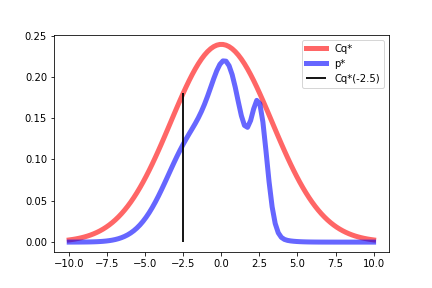
\includegraphics[scale=0.7]{rejection_sampling}
	\caption{Representación gráfica del algoritmo: se samplea un valor para \(\bar{X}\) usando \(q\) y se samplea una uniforme sobre la linea negra, que va desde el 0 hasta \(Cq^\ast(\bar{X})\), y si cae dentro del área de \(p*\) entonces el \(\bar{X}\) es aceptado como muestra de \(p\).}
	\label{fig:rejection_sampling}
\end{figure}
El problema con este método, es que \(q(x)\) debe ser una buena aproximación de \(p(x)\), ya que en caso contrario la constante \(C\) será muy grande y, por ende, la frecuencia de rechazo será muy grande. Además, la constante crece de forma exponencial con el tamaño de la dimensión de \(X(\Omega)\), por lo que no puede ser utilizado en grandes dimensiones.

\subsection{Muestreo por Importancia}

El método muestreo por importancia (llamado \emph{importance sampling} en inglés) no es un método para generar muestras, sino que para estimar la esperanza de una función \(f\) con respecto a \(p(x) = \frac{p^{\ast}(x)}{Z}\), donde solo podemos evaluar \(p^{\ast}(x)\). Supongamos que tenemos una densidad propuesta \(q(x) = \frac{q^{\ast}(x)}{Z_q}\), de la cual podemos obtener muestras y evaluar \(q^{\ast}(x)\). Si \(q(x) > 0\), entonces se cumple la siguiente igualdad: 
\begin{equation*}
\mean_{X}(f) = \int f(x) p(x) \dd{x} = \int f(x) \frac{p(x)}{q(x)} q(x) \dd{x} = \mean_{q}\left(f\frac{p}{q}\right).
\end{equation*}

\begin{figure}[h]
	\centering
	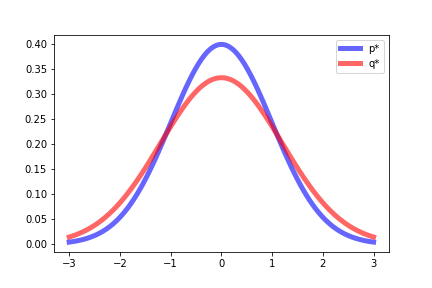
\includegraphics[scale=0.7]{important_sampling}
	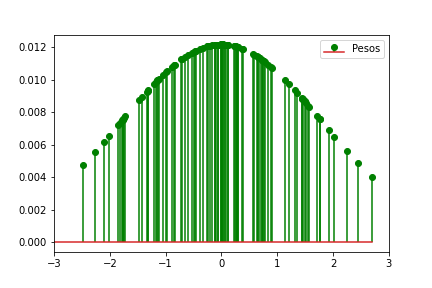
\includegraphics[scale=0.7]{important_sampling_w}
	\caption{Arriba: Las funciones de densidad de distribución objetivo \(p*(x)\) y propuesta \(q*(x)\). Abajo: Los pesos de muestras (samples) de \(q(x)\).}
	\label{fig:important_sampling}
\end{figure}

Sean \(\{X^i\}_{i=1}^N\) \(N\) muestras de \(q(x)\), y definamos sus \emph{pesos} como
\begin{equation*}
w_i = \frac{p^{\ast}(X^i)}{q^{\ast}(X^i)},
\end{equation*}
con los cuales ajustamos la \emph{importancia} de cada punto en nuestro estimador
\begin{equation*}
\hat{\Phi} = \sum_{i=1}^N \frac{w_i}{\sum_{j=1}^N w_j} f(X^i).
\end{equation*}
Para que nuestro estimador \(\hat{\Phi}\) converja a \(\Phi\), es necesario que se cumpla que para todo \(x\), \(p(x) > 0 \implies q(x) > 0\). Idealmente, \(q(x)\) debe parecerse lo más posible a \(p(x)\), incluso en las colas, que deben decrecer a una velocidad similar. El gran problema de este método es que el rango de los pesos \(w_i\) es exponencial a la raíz cuadrada de la dimensión de \(X(\Omega)\):
\begin{equation*}
\frac{w^{\max}}{w^{\mathrm{med}}} = O(\exp(\sqrt{\dim(X(\Omega))})),
\end{equation*}
por lo que la estimación estará dominada por unas pocas muestras con gran peso.

\subsection{Cadenas de Markov de Monte Carlo (MCMC)}

Los métodos anteriores tienen sus ventajas en casos simples, pero su principal desventaja es que no se comportan bien para distribuciones de gran dimensión, ya que es difícil construir una distribución propuesta similar a la distribución objetivo en todas sus dimensiones. 

Un enfoque diferente al problema de inferencia se basa en el mecanismo de cadenas de Markov, en donde los \emph{estados} de la cadena son los conjuntos de valores de las variables a muestrear, y con una función de \emph{transición} de probabilidades adecuada entre estos se procede a muestrear los valores de la cadena. Luego de un cierto tiempo conocido como \emph{burn-in time}, la simulación converge a una distribución \emph{estacionaria} que coincide con la distribución objetivo.

Formalicemos todos estos conceptos a continuación. Por abuso de notación, si el espacio de estados \(\calX\) es discreto o continuo, entonces \(\prob\) denotará la función de masa o de densidad respectivamente.
\begin{definition}
	Una cadena es un proceso estocástico a tiempo discreto con valores en \(\calX\), es decir \((X_n)_{n \in \naturals}\). Decimos que la cadena es de Markov si cumple que para cualquier valor en sus estados \(x_0, x_1, \dotsc, x_n, x_{n+1} \in \calX\) se satisface que
	\[\prob(X_{n+1} = x_{n+1} \mid X_n = x_n, \dotsc, X_0 = x_0) = \prob(X_{n+1} = x_{n+1} \mid X_n = x_n).\]
\end{definition}
Se dice que una cadena de Markov es homogénea si la probabilidad de pasar de un estado a otro, en un paso, no depende del tiempo en que se encuentre la cadena, es decir,
\[\prob(X_{n+1} = b \mid X_n = a) = \prob(X_1 = b \mid X_0 = a) = T(a, b).\]
El kernel \(T\) cumple con que \(T(a, b) \geq 0\) y \(\int_{\calX} T(a, x) \dd{x} = 1\) para todo \(a, b \in \calX\).

Así como \(T(a, b)\) es la probabilidad de llegar desde el estado \(a\) al estado \(b\) en un paso, \(T^n(a, b)\) es la probabilidad de llegar desde el estado \(a\) al estado \(b\) en \(n\) pasos. Notemos que \(T^2(a,b) = \int_\calX T(a, x) T(x, b) \dd{x}\) y \(T^n(a,b) = \int_\calX T^{n-1}(a, x) T(x, b) \dd{x}\).

Diremos que dos estados \(a, b \in \calX\) se comunican si existen \(n_1, n_2 \in \naturals\) tales que \(T^{n_1}(a, b) > 0\) y \(T^{n_2}(b, a) > 0\). Si todos los estados se comunican entre sí, entonces diremos que la cadena es irreducible.

El periodo de un estado \(a \in \calX\) se define como \(d(a) = \mathrm{mcd}\{n \geq : T^n(a, a) > 0\}\), donde \(\mathrm{mcd}\) denota el máximo común divisor. Si \(d(a) = 1\) diremos que el estado \(a\) es aperiódico, y si todos los estados son aperiódicos entonces se dice que la cadena es aperiódica.

La última propiedad de una cadena de Markov que vamos a introducir es la recurrencia positiva. El tiempo medio de recurrencia de un estado \(j\) a partir del estado \(i\) se define como el siguiente valor esperado:
\[\mu_{i, j} = \mean(\min\{n \geq 1 : X_n = j \mid X_0 = i\}).\]
Si \(\mu_{i, i}\) es finito, entonces se dice que \(i\) es recurrente positivo, y si todos los estados son recurrentes positivos entonces se dice que la cadena es recurrente positiva.

Denotemos por \(\pi = (\pi_i)_{i\in\calX}\) a una distribución de probabilidad sobre \(\calX\). Se dice que \(\pi\) es una distribución estacionaria para una cadena de Markov con kernel de \(T\) si se cumple que para \(y \in \calX\),
\[\pi_j = \int_{\calX}T(x, j) \pi_x \dd{x}.\]
Si la cadena de Markov es homogénea con kernel de transición \(T\), irreducible, aperiódica y recurrente positiva, entonces la cadena tiene una única distribución estacionaria \(\pi\) tal que para todo \(i \in \calX\) se tiene que
\[\lim_{n \to \infty} T^n(i, j) = \pi_j.\]

El resultado anterior quiere decir que, dada una distribución de probabilidad \(\prob\), si somos capaces de construir una cadena de Markov con kernel de transición \(T_\prob\) tal que su distribución estacionaria sea \(\prob\), entonces después de simular por un tiempo conocido como \emph{burn-in}, partiendo desde cualquier punto una simulación termina muestreando desde \(\prob\). Veamos a continuación los métodos de MCMC más utilizados.

\subsection{Metropolis-Hasting}

Sea \(\prob(X)\) la distribución de probabilidad de la cual se quiere muestrear \(X = \{x_1, \dotsc, x_n\}\), y sea \(Q(x^{\ast}; x)\) una distribución propuesta para muestrear un valor candidato \(x^{\ast}\) desde el valor actual \(x\).
\begin{figure}[h]
	\centering
	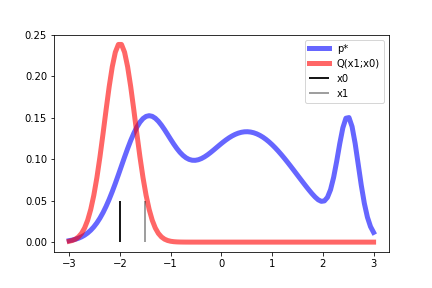
\includegraphics[scale=0.5]{MH1}
	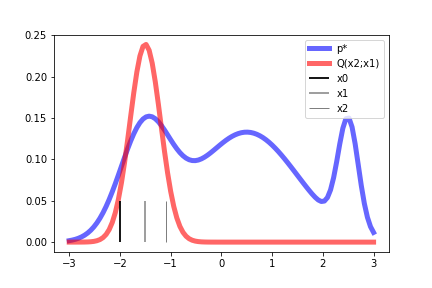
\includegraphics[scale=0.5]{MH2}
	\caption{Izquierda: Primera iteración del método Metropolis-Hasting. Derecha: Segunda iteración del método Metropolis-Hasting.}
	\label{fig:MH}
\end{figure}
Construimos una cadena de Markov que se mueve desde el estado \(x\) al estado \(x^{\ast}\) con una probabilidad de aceptación dada por
\begin{equation*}
A(x, x^{\ast}) = \min \left\{1, \frac{\prob(x^{\ast}) Q(x; x^{\ast})}{\prob(x) Q(x^{\ast}; x)} \right\}.
\end{equation*}
y en caso contrario permanece en \(x\). El algoritmo es muy simple, pero depende completamente de la distribución propuesta \(Q\). A continuación se muestra el seudocódigo del algoritmo general.

\begin{algorithm}[h]
	\caption{Metropolis-Hastings}
	\begin{algorithmic}[1]
		\State Inicializar \(x^{(0)}\).
		\For{\(i = 0, \dotsc, N-1\)}
		\State Muestrear \(u \sim \calU(0, 1)\).
		\State Muestrear \(x^{\ast} \sim Q(x^{\ast}; x^{(i)})\)
		\If{\(u < A(x^{(i)}, x)\)}
		\State \(x^{(i + 1)} \gets x^{\ast}\).
		\Else
		\State \(x^{(i + 1)} \gets x^{(i)}\).
		\EndIf
		\EndFor
	\end{algorithmic}
\end{algorithm}

Para demostrar que este algoritmo converge a la distribución objetivo \(\prob\) basta con demostrar que la cadena construida tiene un kernel de transición \(T\) tal que:
\begin{align*}
T(x, y)				&= Q(y; x) A(x, y),\\
T(x, y) \prob(x)	&= T(y, x) \prob(y).
\end{align*}

En efecto,
\begin{enumerate}
	\item Si \(Q(y; x) \prob(x) = Q(x; y) \prob(y)\), entonces \(A(x, y) = A(y ,x) = 1\) por lo que \(T(x, y) \prob(x) = T(y, x)\prob(y)\).
	
	\item Si \(Q(y; x) \prob(x) > Q(x; y) \prob(y)\), entonces
	\[A(x, y) = \frac{Q(x; y) \prob(y)}{Q(y; x) \prob(x)},\]
	y \(A(y, x) = 1\), lo que implica que
	\begin{align*}
	T(x, y) \prob(x)	&= Q(y; x) A(x, y) \prob(x)\\
	&= Q(y; x) \frac{Q(x; y) \prob(y)}{Q(y; x) \prob(x)} \prob(x)\\
	&= Q(x; y) \prob(y)\\
	&= Q(x; y) A(y, x) \prob(y)\\
	&= T(y, x)\prob(y).
	\end{align*}
	\item Si \(Q(y; x) \prob(x) < Q(x; y) \prob(y)\), entonces \(A(x, y) = 1\) y
	\[A(y, x) = \frac{Q(y; x) \prob(x)}{Q(x; y) \prob(y)},\]
	lo que implica que
	\begin{align*}
	T(y, x) \prob(y)	&= Q(x; y) A(y, x) \prob(y)\\
	&= Q(x; y) \frac{Q(y; x) \prob(x)}{Q(x; y) \prob(y)} \prob(y)\\
	&= Q(y; x) \prob(x)\\
	&= Q(y; x) A(x, y) \prob(x)\\
	&= T(x,y) \prob(x).
	\end{align*}
\end{enumerate}

En el caso particular en que \(Q(y; x)\) es simétrica, entonces el algoritmo se conoce como simplemente \emph{Metropolis} y el cambio es que la función de aceptación es de la forma
\begin{equation*}
A(x^{(i)}, x^{\ast}) = \min \left\{1, \frac{\prob(x^{\ast})}{\prob(x^{(i)})}\right\}.
\end{equation*}

La principal gracia de los métodos de MCMC es que para simular debemos calcular la razón entre las probabilidades \(\prob(x^{\ast})\) y \(\prob(x^{(i)})\), por lo que si tenemos una versión no normalizada \(\hat{\prob}\), la constante de normalización se simplifica al calcular dicha razón, es decir,
\[\frac{\hat{\prob}(x^{\ast})}{\hat{\prob}(x^{(i)})} = \frac{\prob(x^{\ast})}{\prob(x^{(i)})}.\]

\subsection{Muestreo de Gibbs}

Sea \(X = \{x_1, \dotsc, x_n\}\) y definamos \(x_{-i} = X \setminus \{x_i\}\). Supongamos que es posible calcular \(\prob(x_i \mid x_{-i})\) para todo \(i = 1, \dotsc, n\). En ese caso definamos la distribución propuesta
\[ Q(x^{\ast}; x^{(i)}) = \begin{dcases*}
\prob(x_j^{\ast} \mid x_{-j}^{(i)})	& si \(x_{-j}^{\ast} = x_{-j}^{(i)}\),\\
0									& en caso contrario.
\end{dcases*} \]

El Muestreo de Gibbs es el caso particular de Metropolis-Hasting, con la distribución recién definida, y cumple que su probabilidad de aceptación es:
\begin{align*}
A(x^{(i)}, x^{\ast})	&= \min \left\{1, \frac{\prob(x^{\ast})Q(x^{(i)}; x^{\ast})}{\prob(x^{(i)}) Q(x^{\ast}; x^{(i)})} \right\}\\
&= \min \left\{1, \frac{\prob(x^{\ast}) \prob(x_j^{(i)} \mid x_{-j}^{(i)})}{\prob(x^{(i)}) \prob(x_j^{\ast} \mid x_{-j}^{\ast})} \right\}\\
&= \min \left\{1, \frac{\prob(x_{-j}^{\ast})}{\prob(x_{-j}^{(i)})} \right\}\\
&= 1.
\end{align*}
Esto quiere decir que todo algoritmo que muestree generado en cada iteración es aceptado. La selección de la variable a muestrear se puede hacer de forma ordenada o de forma aleatoria. A continuación mostramos el algoritmo para el caso ordenado:
\begin{algorithm}[h]
	\caption{Muestreo de Gibbs Ordenado}
	\begin{algorithmic}[1]
		\State Inicializar \(x^{(0)}\).
		\For{\(i = 0, \dotsc, N-1\)}
		\For{\(j = 1, \dotsc n\)}
		\State Muestrear \(x_j^{(i+1)} \sim \prob(x_j \mid x_{-j}^{(i)})\).
		\EndFor
		\EndFor
	\end{algorithmic}
\end{algorithm}

En \cite{green1995reversible} se propone un método MCMC aplicado a la modelación bayesiana, que permite saltar de dimensión en la cantidad de parámetros de la cadena, lo que es muy útil si no se conocen a priori la cantidad de parámetros a estimar. En \cite{murray2008gaussian} se presenta un método de MCMC en donde se modela una distribución utilizando un GP auxiliar, permitiendo así modelar las distribuciones de forma bayesiana y no paramétrica.
\comment{seccion: quizas falta un ejemplo simplecito para entender}

\comment{parrafo: pequeña reseña y aterrizado de lo enseñado}

\comment{parrafo: dado que es un tema bien conocido por donzas, un parrafo motivando otras lecturas y menciones del estado del arte.}

\subsection{Inferencia Variacional}

\comment{Parrafo: contexto, mostrarlo como una alternativa a MCMC}

Las técnicas de inferencia variacional se basan en aproximar la distribución condicional \(p(\theta \mid X)\) utilizando una distribución variacional \(q(\theta)\) que maximice la similitud con la distribución\ \(p(\theta \mid X)\) con el criterio de la divergencia de Kullback-Leibler, de forma que
\begin{equation*}
\argmin_{q} \KL (q \parallel p(\cdot \mid X)) = \int  \ln \left(\frac{q(\theta)}{p(\theta \mid X)}\right) q(\theta)\dd{\theta}.
\end{equation*}
Se puede comprobar la siguiente relación:
\begin{equation*}
\ln p(X) = \KL (q \parallel p(\cdot \mid X)) + F(q, X).
\end{equation*}
Luego, para minimizar \(\KL\) se debe maximizar la energía libre \(F\):
\begin{equation*}
F(q, X) = \int q(\theta) \ln \left(\frac{p(\theta, X)}{q(\theta)}\right) \dd{\theta} = \left\langle \ln p(\cdot, X) \right\rangle_{q} + H(q),
\end{equation*}
donde \(H(q)\) es la entropía de \(q\), y \(\left\langle \ln p(\theta,X) \right\rangle_q\) es la \emph{expected log-joint}. 

Un ejemplo simple es la conocida aproximación de Laplace, que se describe a continuación:
\begin{align*}
\theta^{\ast}	&= \argmax_{\theta} \ln p(\theta,X),\\
\Lambda			&= \nabla_\theta \nabla_\theta \ln p(\theta^{\ast},X),\\
q(\theta)		&\sim \calN(\theta \mid \theta^{\ast}, \Lambda^{-1}).
\end{align*}
Se puede revisar \cite{titsias2009variational}, \cite{gal2014variational}, y \cite{matthews2016sparse} para profundizar en el tema de las aplicaciones de inferencia variacional a procesos gaussianos.
\comment{expandir más este ultimo parrafo, motivando la lectura de otras cosas asi como avances recientes, la idea es que el libro tambien pueda ser una guia a los que quieran profundizar más.}